% Created 2015-03-19 Thu 18:27
\documentclass[11pt]{article}
\usepackage[utf8]{inputenc}
\usepackage{lmodern}
\usepackage[T1]{fontenc}
\usepackage{fixltx2e}
\usepackage{graphicx}
\usepackage{longtable}
\usepackage{float}
\usepackage{wrapfig}
\usepackage{rotating}
\usepackage[normalem]{ulem}
\usepackage{amsmath}
\usepackage{textcomp}
\usepackage{marvosym}
\usepackage{wasysym}
\usepackage{amssymb}
\usepackage{amsmath}
\usepackage[version=3]{mhchem}
\usepackage[numbers,super,sort&compress]{natbib}
\usepackage{natmove}
\usepackage{url}
\usepackage{minted}
\usepackage{underscore}
\usepackage[linktocpage,pdfstartview=FitH,colorlinks,
linkcolor=blue,anchorcolor=blue,
citecolor=blue,filecolor=blue,menucolor=blue,urlcolor=blue]{hyperref}
\usepackage{attachfile}
\usepackage[left=1in, right=1in, top=1in, bottom=1in, nohead]{geometry}
\usepackage{hyperref}
\usepackage{setspace}
\usepackage[labelfont=bf]{caption}
\usepackage{amsmath}
\usepackage{enumerate}
\usepackage[parfill]{parskip}
\author{Prateek Mehta, William F. Schneider}
\date{2015-01-22 Thu}
\title{Computational Chemistry Laboratory I (CBE 60547)}
\begin{document}

\maketitle

\section{Introduction to Linux}
\label{sec-1}

Much of the work in this course will involve some use of the unix terminal. Mac and Linux users can access the terminal from their applications menu. Windows users will probably need to use putty to login to the CRC machines to use a linux environment.

\subsection{Logging onto the CRC}
\label{sec-1-1}

Windows Users: Open putty, login. 

Mac/Linux Users: Open the terminal and type: 

\begin{minted}[frame=lines,fontsize=\scriptsize,linenos]{sh}
ssh -Y username@crcfe01.crc.nd.edu
\end{minted}


\subsection{Common Linux Commands}
\label{sec-1-2}

Here is a list of common linux commands, along with an example of their output. Try typing these in your terminal window.

\begin{itemize}
\item \verb~ls~: List the contents of a directory
\end{itemize}

\begin{minted}[frame=lines,fontsize=\scriptsize,linenos]{sh}
ls
\end{minted}

\begin{verbatim}
FDA
images
lab1.org
lab1.pdf
Lab1.png
lab1.tex
\end{verbatim}

\begin{itemize}
\item \verb~pwd~: Get the path of the current directory
\end{itemize}

\begin{minted}[frame=lines,fontsize=\scriptsize,linenos]{sh}
pwd
\end{minted}

\begin{verbatim}
/afs/crc.nd.edu/user/p/pmehta1/computational-chemistry/Lab1
\end{verbatim}

\begin{itemize}
\item \verb~mkdir~: Create a directory
\end{itemize}

\begin{minted}[frame=lines,fontsize=\scriptsize,linenos]{sh}
mkdir example-directory
ls
\end{minted}

\begin{verbatim}
example-directory
FDA
images
lab1.org
lab1.pdf
Lab1.png
lab1.tex
\end{verbatim}

\begin{itemize}
\item \verb~cd~: Change directory
\end{itemize}

\begin{minted}[frame=lines,fontsize=\scriptsize,linenos]{sh}
cd example-directory
pwd
cd .. # move 1 directory up
pwd
\end{minted}

\begin{verbatim}
/afs/crc.nd.edu/user/p/pmehta1/computational-chemistry/Lab1/example-directory
/afs/crc.nd.edu/user/p/pmehta1/computational-chemistry/Lab1
\end{verbatim}

\begin{itemize}
\item \verb~cp~ Copy files
\end{itemize}
\begin{minted}[frame=lines,fontsize=\scriptsize,linenos]{sh}
cp file1 file2
\end{minted}


\begin{itemize}
\item \verb~mv~: Move files
\end{itemize}
\begin{minted}[frame=lines,fontsize=\scriptsize,linenos]{sh}
mv file1 file2
\end{minted}

\begin{itemize}
\item \verb~rm~: Remove files
\end{itemize}
\begin{minted}[frame=lines,fontsize=\scriptsize,linenos]{sh}
rm filename
\end{minted}

\begin{itemize}
\item \verb~quota~: Check the amount of space allocated to you by the CRC.
\end{itemize}

\begin{minted}[frame=lines,fontsize=\scriptsize,linenos]{sh}
quota
\end{minted}

\begin{verbatim}
AFS quota using values reported by vos server for partition
Quota for /afs/crc.nd.edu/user/p/pmehta1 
Volume Name                   Quota      Used %Used   Partition
u.pmehta1                    100 GB     55 GB   55%         87%
\end{verbatim}


\subsection{Obtaining lab notes}
\label{sec-1-3}

The lab notes and homeworks can be obtained from the course website. They are also conveniently stored in a git repository. To obtain the files just type in

\begin{minted}[frame=lines,fontsize=\scriptsize,linenos]{sh}
git clone https://github.com/wfschneidergroup/computational-chemistry
\end{minted}

You can periodically update your copy of the notes by changing into the course directory and running the command \verb~git pull~, i.e.,

\begin{minted}[frame=lines,fontsize=\scriptsize,linenos]{sh}
cd computational-chemistry
git pull
\end{minted}


\section{The very least you have to know about GNU Emacs}
\label{sec-2}

For the purposes of this course, we will use GNU Emacs as our text editor, and in particular Emacs org-mode. Getting started with it can be a little challenging, but learning how to use it offers many benefits, which we shall soon see. If you really, really want to use another editor, you are free to do so, but it is likely that you will lose some customized emacs features which will help you with this course.

Here are a few things to get started.

\begin{itemize}
\item Starting Emacs. To start emacs type \verb~emacs &~ on the command line. This will launch emacs with the jmax starter kit (\url{https://github.com/jkitchin/jmax}). You can add your own customizations when you start learning more.

\item The first screen you will see is called the scratch buffer. It is mainly for doing temporary things that are not generally required to be saved.

\item Emacs is built around modifier keys, e.g., <Control>, <Alt>, <Shift>, <Esc>. These keys allow you to give instructions to emacs, e.g. keyboard shortcuts to open a file, close a file, run a command, etc. The commands are usually are in the form of <modifier key><some letter>.

\item To create a new file, click on the file menu and select \texttt{visit new file}. This will prompt you to enter the filename at the small window at bottom of the screen. This small window is called the mini-buffer. Create a file \texttt{test.org}.

\item An alternate way to open a file (or create a new file if it does not exist) is to type \verb~Control-x Control-f~ (or \verb~C-x C-f~ in Emacs notation). It should bring up the same prompt to enter the filename in your mini-buffer.

\item Once your file is open, you can try typing something in it. Now save your file. You can do this from the file menu or using the command, \verb~C-x C-s~.

\item Cut/Copy/Paste. The biggest difference between Emacs and other text editors is how to cut, copy and paste text. We can use the edit menu to do this, or use the short cuts,

\begin{itemize}
\item \verb~C-w~. Cut selected text.
\item \verb~M-x~. Copy selected text. (Here M is the \texttt{Alt} key for windows/linux users, the \texttt{Command} key for Mac users)
\item \verb~C-y~. Paste cut/copied text.
\end{itemize}

\item To close emacs, you can click on the 'X' sign on the corner of your screen or type, \verb~C-x C-c~.

\item Now that you are back at your terminal, use emacs to open the notes for today's lab. Change into the the directory you just cloned, and type \verb~emacs lab1.org &~. This is the org-mode file that was used to create the pdf. All the commands that you just ran in the terminal were run inside this document!

\item Press <TAB> to expand the headings and see what they contain. Navigate to this section of the document.

\item Finally, we will consider how to run an emacs command, namely one that will make the equations in the document readable. Type \verb~M-x~. Now type \verb~org-toggle-latex-overlays~. Alternately, you can click on this link, \url{org-toggle-latex-overlays}. You should be able to see the Schrodinger equation below.

\item $H\psi = E\psi$

\item \textbf{Tip:} If you find yourself stuck somewhere, type <ESC> four times or type \verb~C-g~.
\end{itemize}


\section{Introduction to Python}
\label{sec-3}

Python is a programming language which we will use to solve many of the homework problems, especially density functional theory calculations using VASP (homeworks 5, homework 6, and probably your class project). It is therefore important that you familiarize yourself with using it. The numerical and plotting features in python are mostly similar to \texttt{MATLAB}, with a few subtle differences. I would recommend that you try to solve the first problem in homework 2 using python. A few examples are below, adapted (a fancy way of saying pretty much copied) from John Kitchin's example files. We won't cover all of these, but you can use them for reference. To execute a code block type \verb~C-c C-c~.

\subsection{Simple calculations}
\label{sec-3-1}

A good overview of basic python operators can be found at \url{http://www.tutorialspoint.com/python/python_basic_operators.htm}

Here are some simple examples
\begin{minted}[frame=lines,fontsize=\scriptsize,linenos]{python}
print 2+3
print 4-6
print 2*7
print 4.0 / 6.0
\end{minted}

\begin{verbatim}
5
-2
14
0.666666666667
\end{verbatim}


Division is a little tricky. Python distinguishes between integer division and float division. In the first line we have integer division, where the remainder is discarded and an integer is returned. If any number is a float (indicated by a decimal or because it is converted to a float) then a float is returned.

\begin{minted}[frame=lines,fontsize=\scriptsize,linenos]{python}
print 2/3
print 2./3.
print 2/3.
print 2/float(3)  # the float function casts the integer to a float
\end{minted}

\begin{verbatim}
0
0.666666666667
0.666666666667
0.666666666667
\end{verbatim}

\begin{minted}[frame=lines,fontsize=\scriptsize,linenos]{python}
print 2*3
print 2*3.0
\end{minted}

\begin{verbatim}
6
6.0
\end{verbatim}

We can also do powers with \texttt{**}

\begin{minted}[frame=lines,fontsize=\scriptsize,linenos]{python}
print 2**3
print 2**0.5
print 2^4    # Binary XOR operator!
\end{minted}

\begin{verbatim}
8
1.41421356237
6
\end{verbatim}

The modulus operator (\%) divides the left hand operand by the right hand operand and returns the remainder.

\begin{minted}[frame=lines,fontsize=\scriptsize,linenos]{python}
print 5 % 4
print 5. % 4.
\end{minted}

\begin{verbatim}
1
1.0
\end{verbatim}


\subsection{Formatted printing}
\label{sec-3-2}
\url{http://docs.python.org/library/stdtypes.html#string-formatting-operations}

We will usually want to print more than a number, e.g. some descriptive text and the number. We also will want to format numbers so we do not see 9 decimal places all the time. We use string formatting for that. Here are some typical examples.

In a string we can specify where to put numbers with positional arguments like \{0\}. That says take the first argument (python starts counting at zero) and put it in place of \{0\}.

\begin{minted}[frame=lines,fontsize=\scriptsize,linenos]{python}
a = 4.5 + 2
print 'The answer is {0}'.format(a)
\end{minted}

\begin{verbatim}
The answer is 6.5
\end{verbatim}


We can have more than one number to format like this.
\begin{minted}[frame=lines,fontsize=\scriptsize,linenos]{python}
a = 5**3
b = 23
print 'a = {1} and b = {0}'.format(b,a)
\end{minted}

\begin{verbatim}
a = 125 and b = 23
\end{verbatim}

Alternatively, we can use named arguments to specify the values. It is your choice which one to do. Named arguments require more typing, but are easier to understand.
\begin{minted}[frame=lines,fontsize=\scriptsize,linenos]{python}
a = 5**3
b = 23
print 'a = {ans0} and b = {ans1}'.format(ans0=a,
                                         ans1=b)
\end{minted}

\begin{verbatim}
a = 125 and b = 23
\end{verbatim}

To do formatting, we need additional syntax. We use \{i:format\} to specify how the value should be formatted. Here we show how to specify only three decimal places on a results. See \href{http://docs.python.org/library/stdtypes.html#string-formatting-operations}{this link} for a lot more details of formatting strings.
\begin{minted}[frame=lines,fontsize=\scriptsize,linenos]{python}
a = 2./3.
print 'a = {0}'.format(a)
print 'a = {0:1.3f}'.format(a)
\end{minted}

\begin{verbatim}
a = 0.666666666667
a = 0.667
\end{verbatim}


\subsection{Data types}
\label{sec-3-3}
Numeric types \url{http://docs.python.org/library/stdtypes.html#numeric-types-int-float-long-complex}

Strings \url{http://docs.python.org/library/stdtypes.html#string-methods}


\subsubsection{lists/tuples}
\label{sec-3-3-1}

Lists and tuples are similar in that they are both sets of data. A list is delimited by [] (square brackets) and a tuple is delimited by () (parentheses). The difference between them is a list can be changed after it is created (it is mutable), but a tuple cannot (it is immutable).

\begin{minted}[frame=lines,fontsize=\scriptsize,linenos]{python}
# short list example
a = [1, 2, 3, 4] # a list
print a
print len(a)
print a[0] # first element
print a[-1] # last element
print a[3]  # also last element
print 2*a   # surprise!!!
\end{minted}

\begin{verbatim}
[1, 2, 3, 4]
4
1
4
4
[1, 2, 3, 4, 1, 2, 3, 4]
\end{verbatim}

We can create a list with the \texttt{range} command:

\begin{minted}[frame=lines,fontsize=\scriptsize,linenos]{python}
a = range(4)
print a

b = range(4,10)
print b

print a + b  # surprise again!!!
\end{minted}

\begin{verbatim}
[0, 1, 2, 3]
[4, 5, 6, 7, 8, 9]
[0, 1, 2, 3, 4, 5, 6, 7, 8, 9]
\end{verbatim}

Note that algebraic/math operations are not defined for lists the way they are for Matlab. We have to use \texttt{numpy.array} for that, which we will see later.

\begin{minted}[frame=lines,fontsize=\scriptsize,linenos]{python}
# short list example
a = [1, 2, 3, 4] # a list
print a
a[1] = 56 # change the value of 2nd element
print a
\end{minted}

\begin{verbatim}
[1, 2, 3, 4]
[1, 56, 3, 4]
\end{verbatim}

Tuples are like lists except they cannot be modified after creation.

\begin{minted}[frame=lines,fontsize=\scriptsize,linenos]{python}
a = (1,2,3,4)
print len(a)
print a[0]
print a[-1]
a[1] = 56 #this is not allowed!
\end{minted}


\subsection{Conditional statements}
\label{sec-3-4}
conditional operators \url{http://docs.python.org/library/stdtypes.html#comparisons}

Python has the standard conditional operators for testing if a quantity is equal to (\texttt{=), less than (<), greater than (>), lessthan or equal to (<}) greater than or equal to (>=) and not equal (!=). These generally work on numbers and strings.

\begin{minted}[frame=lines,fontsize=\scriptsize,linenos]{python}
print 4 == 2.
print 'a' != 'A'
print 4 > 3
print 4 <= 3
print 'a' < 'b' # hmmm....
\end{minted}

\begin{verbatim}
False
True
True
False
True
\end{verbatim}

We use these conditional operators to determine whether conditional statements should be run or not.

\begin{minted}[frame=lines,fontsize=\scriptsize,linenos]{python}
a = 4
b = 5

if a < b:
    print 'a is less than b'
\end{minted}

\begin{verbatim}
a is less than b
\end{verbatim}

In this next example we use an \texttt{else} statement. Note the logic is not complete, if a=b in this case, we would get the statement "a is less than b" printed.
\begin{minted}[frame=lines,fontsize=\scriptsize,linenos]{python}
a = 14
b = 5

if a > b:
    print 'a is greater than b'
else:
    print 'a is less than b'
\end{minted}

\begin{verbatim}
a is greater than b
\end{verbatim}

Here is a more complete logic that uses \texttt{elif} to add an additional logic clause.
\begin{minted}[frame=lines,fontsize=\scriptsize,linenos]{python}
a = 4
b = 4
if a > b:
    print 'a is greater than b'
elif a == b:
    print 'a is equal to b'
else:
    print 'a is less than b'
\end{minted}

\begin{verbatim}
a is equal to b
\end{verbatim}

Finally, to illustrate that the first conditional statement that evaluates to True is evaluated, consider this example:
\begin{minted}[frame=lines,fontsize=\scriptsize,linenos]{python}
a = 4
b = 4
if a > b:
    print 'a is greater than b'
elif a >= b:
    print 'a is greater than or equal to b'
elif a == b:
    print 'a is equal to b'
elif a <= b:
    print 'a is less than or equal to b'
else:
    print 'a is less than b'
\end{minted}

\begin{verbatim}
a is greater than or equal to b
\end{verbatim}


\subsection{Loops}
\label{sec-3-5}
\url{http://docs.python.org/tutorial/datastructures.html#looping-techniques}
for
while/break/continue
enumerate, zip

\begin{minted}[frame=lines,fontsize=\scriptsize,linenos]{python}
for i in [0,1,2,3]:
    print i


for i in range(4):
    print i
\end{minted}

\begin{verbatim}
0
1
2
3
0
1
2
3
\end{verbatim}


\subsection{functions}
\label{sec-3-6}
\url{http://docs.python.org/tutorial/controlflow.html#defining-functions}

We can define functions with the \texttt{def} statement, and specify what they \texttt{return}
\begin{minted}[frame=lines,fontsize=\scriptsize,linenos]{python}
def myfunc(x):
    return x*x

print myfunc(3)
print myfunc(x=3)
\end{minted}

\begin{verbatim}
9
9
\end{verbatim}


\subsection{Classes and objects}
\label{sec-3-7}
\url{http://docs.python.org/tutorial/classes.html}


\subsection{Modules}
\label{sec-3-8}
\url{http://docs.python.org/tutorial/modules.html}

The default Python environment has minimal functionality. We can \texttt{import} additional functionality from modules. The full standard library is documented at \url{http://docs.python.org/library/}. It is not likely you will use everything there, but it is helpful to be familiar with what is available so you do not reinvent solutions.

We import modules, and then we can access functions inthe module with the \texttt{.} operator.

\begin{minted}[frame=lines,fontsize=\scriptsize,linenos]{python}
# list contents of current directory
import os
for item in os.listdir('.'):
    print item
\end{minted}

\begin{verbatim}
lab1.org
lab1.pdf
lab1.tex
\end{verbatim}

You can import exactly what you need also with the \texttt{from/import} syntax
\begin{minted}[frame=lines,fontsize=\scriptsize,linenos]{python}
# list contents of current directory
from os import listdir
for item in listdir('.'):
    print item
\end{minted}

\begin{verbatim}
lab1.org
lab1.pdf
lab1.tex
\end{verbatim}

Finally, you can change the name of a module. This may be done for readability, or to shorten the amount of typing.
\begin{minted}[frame=lines,fontsize=\scriptsize,linenos]{python}
# list contents of current directory
import os as operating_system
for item in operating_system.listdir('.'):
    print item
\end{minted}

\begin{verbatim}
lab1.org
lab1.pdf
lab1.tex
\end{verbatim}

\subsubsection{Some common standard modules}
\label{sec-3-8-1}
\url{http://docs.python.org/tutorial/stdlib.html}
os, sys, glob,  re


\subsection{file I/O}
\label{sec-3-9}
reading, writing files
\url{http://docs.python.org/library/stdtypes.html#file-objects}


\subsection{Error handling}
\label{sec-3-10}
\url{http://docs.python.org/tutorial/errors.html}

Errors happen, and when they do they usually kill your script. Sometimes that is not desirable, and it is nice to catch errors, handle them, and keep on going. When errors occur in python, an Exception is raised. We can use \texttt{try/except} code blocks to try some code, and then respond to any exceptions that occur.

\begin{minted}[frame=lines,fontsize=\scriptsize,linenos]{python}
try:
    1/0
except ZeroDivisionError, e:
    print e
    print 'an error was found'
\end{minted}

\begin{verbatim}
integer division or modulo by zero
an error was found
\end{verbatim}


\subsection{Numerical Python (Numpy)}
\label{sec-3-11}

\subsubsection{The basics}
\label{sec-3-11-1}
\url{http://docs.scipy.org/doc/numpy/reference/}

\begin{minted}[frame=lines,fontsize=\scriptsize,linenos]{python}
import numpy as np
a = np.array([1,2,3,8])

print a*a          # element-wise operation
print np.dot(a,a)  # linear-algebra dot product
\end{minted}

\begin{verbatim}
[ 1  4  9 64]
78
\end{verbatim}

Numpy defines lots of functions that operate element-wise on arrays.

\begin{minted}[frame=lines,fontsize=\scriptsize,linenos]{python}
import numpy as np
a = np.array([1, 2, 3, 4])
print a**2
print np.sin(a)
print np.exp(a)
print np.sqrt(a)
\end{minted}

\begin{verbatim}
[ 1  4  9 16]
[ 0.84147098  0.90929743  0.14112001 -0.7568025 ]
[  2.71828183   7.3890561   20.08553692  54.59815003]
[ 1.          1.41421356  1.73205081  2.        ]
\end{verbatim}

\begin{minted}[frame=lines,fontsize=\scriptsize,linenos]{python}
import numpy as np
a = np.array([1, 2, 3, 4])
print a.min(), a.max()
print a.sum()  # sum of elements
print a.mean() # average
print a.std()  # standard deviation
\end{minted}

\begin{verbatim}
1 4
10
2.5
1.11803398875
\end{verbatim}


Below are some recipes for doing linear algebra and polynomials.


\subsubsection{Linear algebra}
\label{sec-3-11-2}
\texttt{numpy.linalg} provides a lot of the linear algebra functionality we need. See \url{http://docs.scipy.org/doc/numpy/reference/routines.linalg.html} for details of all the things that are possible. For example, given these linear equations:

$x + y = 3$, 
$x - y = 1$

we can represent these equations in matrix form $A x = b$ and solve them.

\begin{minted}[frame=lines,fontsize=\scriptsize,linenos]{python}
import numpy as npx
import numpy.linalg as la

A = np.array([[1, 1],
              [1, -1]])

b = np.array([3, 1])

print la.solve(A, b)
\end{minted}

\begin{verbatim}
[ 2.  1.]
\end{verbatim}

You might be familiar with the following solution:

$x = A^{-1} b$

We can also compute that:

\begin{minted}[frame=lines,fontsize=\scriptsize,linenos]{python}
import numpy as np
import numpy.linalg as la

A = np.array([[1, 1],[1, -1]])
b = np.array([3, 1])

print np.dot(la.inv(A), b)
\end{minted}

\begin{verbatim}
[ 2.  1.]
\end{verbatim}

Finally, we can do linear least squares easily. Suppose we have these three equations, and two unknowns:

$x + y = 3$,

$x - y = 1$,

$x - y = 0.9$

\begin{minted}[frame=lines,fontsize=\scriptsize,linenos]{python}
import numpy as np
import numpy.linalg as la

A = np.array([[1, 1],
              [1, -1],
              [1, -1]])
b = np.array([3, 1, 0.9])

[x, residuals, rank, s] = la.lstsq(A,b)
print x
\end{minted}

\begin{verbatim}
[ 1.975  1.025]
\end{verbatim}


\subsubsection{Polynomials}
\label{sec-3-11-3}
\texttt{numpy} can do polynomials too. We express polynomials by the coefficients in front of the powers of $x$, e.g. $4 x^2 + 2x - 1 = 0$ is represented by [4, 2, -1].

\begin{minted}[frame=lines,fontsize=\scriptsize,linenos]{python}
import numpy as np
p = [4, 2, -1]
print np.roots(p)
\end{minted}

\begin{verbatim}
[-0.80901699  0.30901699]
\end{verbatim}

\begin{minted}[frame=lines,fontsize=\scriptsize,linenos]{python}
import numpy as np
p = [4, 2, -1]
print np.polyder(p) # coefficients of the derivative
print np.polyint(p)
\end{minted}

\begin{verbatim}
[8 2]
[ 1.33333333  1.         -1.          0.        ]
\end{verbatim}

We can also readily evaluate polynomials at specific points:
\begin{minted}[frame=lines,fontsize=\scriptsize,linenos]{python}
import numpy as np
p = [4,2,-1]
print np.polyval(p,[0, 1, 2])
\end{minted}

\begin{verbatim}
[-1  5 19]
\end{verbatim}

Polynomials are very convenient functions to fit to data. the \texttt{numpy.polyfit} command does this, and returns the coefficients.

\begin{minted}[frame=lines,fontsize=\scriptsize,linenos]{python}
import numpy as np
x = [0, 2, 3, 4]
y = [1, 5, 7, 9]
p = np.polyfit(x, y, 1)
print 'slope = {0}\nintercept = {1}'.format(*p)
print p
\end{minted}

\begin{verbatim}
slope = 2.0
intercept = 1.0
[ 2.  1.]
\end{verbatim}


\subsection{Scientific Python (Scipy)}
\label{sec-3-12}
\url{http://docs.scipy.org/doc/scipy/reference/}

\texttt{scipy} provides all the functionality we need for \href{http://docs.scipy.org/doc/scipy/reference/tutorial/integrate.html}{integration}, \href{http://docs.scipy.org/doc/scipy/reference/tutorial/optimize.html}{optimization}, \href{http://docs.scipy.org/doc/scipy/reference/tutorial/interpolate.html}{interpolation}, \href{http://docs.scipy.org/doc/scipy/reference/tutorial/stats.html}{statistics}, and \href{http://docs.scipy.org/doc/scipy/reference/tutorial/io.html}{File I/O}. You should look up the link on integration. It might be useful for homework 2.


\subsubsection{Solving Equations}
\label{sec-3-12-1}
Here is a typical usage for solving the equation $x^2 = 2$ for $x$. We have to define a function that is $f(x) = 0$, and then use the \texttt{scipy.optimize.fsolve} function to solve it with an initial guess.

\begin{minted}[frame=lines,fontsize=\scriptsize,linenos]{python}
from scipy.optimize import fsolve

def f(x):
    y = 2 - x**2
    return y

x0 = 1.4 # Intitial Guess
x = fsolve(f, x0)
print x
print type(x)
\end{minted}

\begin{verbatim}
[ 1.41421356]
<type 'numpy.ndarray'>
\end{verbatim}



\subsubsection{Integration Example}
\label{sec-3-12-2}

\begin{enumerate}
\item Using Quad
\label{sec-3-12-2-1}
\begin{minted}[frame=lines,fontsize=\scriptsize,linenos]{python}
from scipy.integrate import quad
import numpy as np

def integrand(x):
    return (1 - np.cos(x))**2

ans, err = quad(integrand, 0, 2)
print ans
\end{minted}

\begin{verbatim}
0.992204522522
\end{verbatim}


\item Using trapz
\label{sec-3-12-2-2}

\begin{minted}[frame=lines,fontsize=\scriptsize,linenos]{python}
import numpy as np

# Array of 100 points between 0 and 2
x2 = np.linspace(0, 2, 100)
y2 = x2**3

print np.trapz(y2, x2)
\end{minted}

\begin{verbatim}
4.00040812162
\end{verbatim}
\end{enumerate}


\subsection{Plotting with Python (Matplotlib)}
\label{sec-3-13}
\url{http://matplotlib.sourceforge.net/}
\texttt{matplotlib} is the prime plotting module for python. The syntax is similar to Matlab. The best way to learn matplotlib is to visit the gallery (\url{http://matplotlib.sourceforge.net/gallery.html}) and look for examples that do what you want. Here is a simple example.

\begin{minted}[frame=lines,fontsize=\scriptsize,linenos]{python}
import numpy as np
import matplotlib.pyplot as plt

x = np.linspace(0,2*np.pi)
y = np.sin(x)

plt.plot(x,y)
plt.plot(x,np.cos(x))
plt.xlabel('X axis')
plt.ylabel('Y axis')
plt.legend(['sin(x)', 'cos(x)'], loc='best')
plt.savefig('images/Lab1.png')
plt.show()
\end{minted}

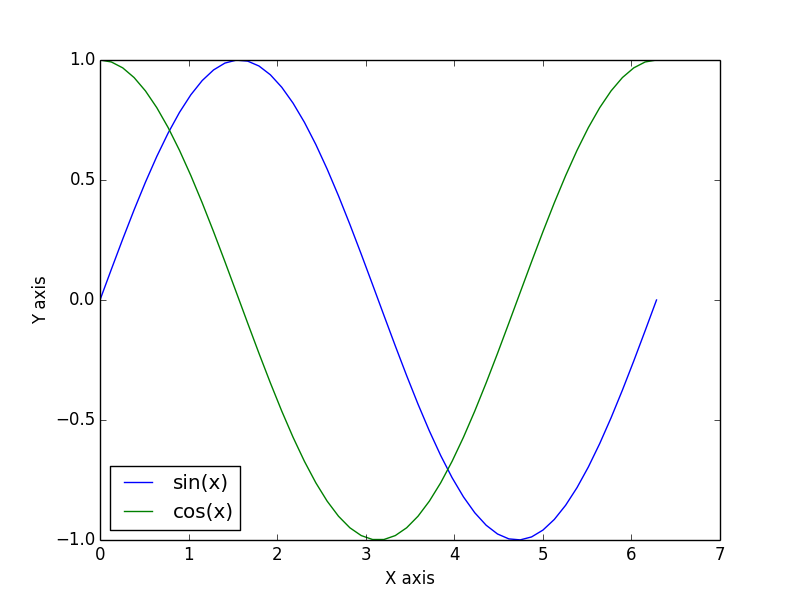
\includegraphics[width=.9\linewidth]{./images/Lab1.png}


\section{FDA}
\label{sec-4}

Now let us run our first computational chemistry code. Change into the \verb~computational-chemistry/Lab1/FDA/fda~ directory and run the command,

\begin{minted}[frame=lines,fontsize=\scriptsize,linenos]{sh}
./fda Ar
\end{minted}

This will use the \texttt{Ar.inp} file as input and produce two output files, \texttt{Ar.dmp} and \texttt{Ar.out}. The \texttt{00READ.ME} file contains some information about the format of the input file. You can open these files with Emacs to read what they contain.

\subsection{Parsing the dmp file}
\label{sec-4-1}

In homework 2, you will need to parse the \texttt{.dmp} file to plot some data. It contains the radial grid values and total charge density in two columns, followed by the charge density of each oribital on the same grid. Here we consider an example of how to do this with python.

\begin{minted}[frame=lines,fontsize=\scriptsize,linenos]{python}
import matplotlib.pyplot as plt
import numpy as np

# Lets open the file in read mode
with open('FDA/fda/Ar.dmp', 'r') as f:

    # Reading all the lines in the file
    # Each line is stored as an element of a list
    lines = f.readlines()

    # First we read the grid points and the total charge densities
    grid_points = []
    total_charge_densities = []

    for line in lines[3:303]:

        # Each is a string with two columns
        grid_point, tot_charge_density = line.split()

        # We need to convert each line to a float add it to our lists
        grid_points.append(float(grid_point))
        total_charge_densities.append(float(tot_charge_density))
    
    # Now for the 1s orbital
    one_s_charge_density = []
    
    for x in lines[304:604]:
        one_s_charge_density.append(float(x))
 
    # Alternately,
    one_s_charge_density_alt = [float(x) for x in lines[304:604]]

plt.figure()
plt.semilogx(grid_points, total_charge_densities)
plt.xlabel('Grid Points')
plt.ylabel('Charge Density')
plt.title('Overall')
plt.savefig('images/Ar-overall-charge-density.png')

plt.figure()
plt.semilogx(grid_points, one_s_charge_density)
plt.xlabel('Grid Points')
plt.ylabel('Charge Density')
plt.title('1s orbital')
plt.savefig('images/Ar-1s-charge-density.png')
plt.show()
\end{minted}

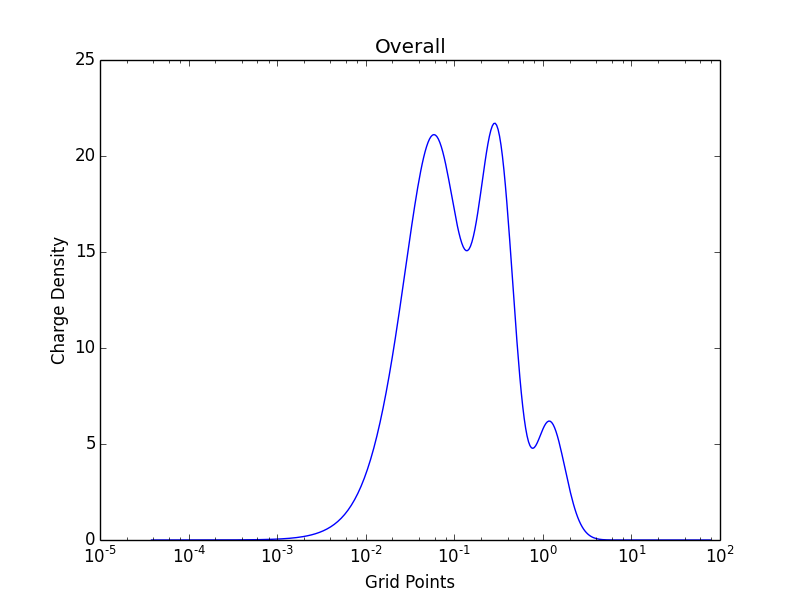
\includegraphics[width=.9\linewidth]{./images/Ar-overall-charge-density.png}

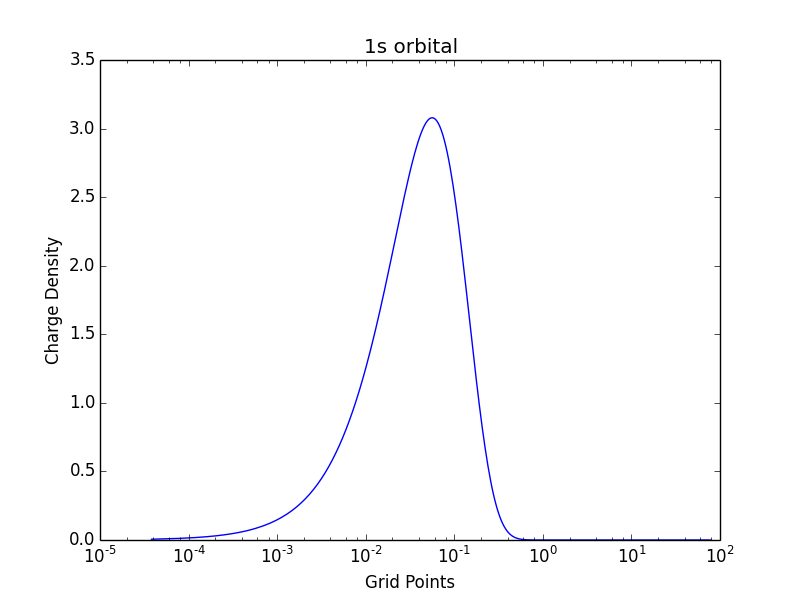
\includegraphics[width=.9\linewidth]{./images/Ar-1s-charge-density.png}
% Emacs 24.4.3 (Org mode 8.2.10)
\end{document}